\chapter{第12套试卷——参考答案与评分标准}

\section{一、选择题答案（18分）}

\begin{enumerate}[label=\arabic*.]

\item \textbf{【答案】B} \quad（3分）\\
\textbf{解析：}基于SRAM工艺的FPGA，配置数据存储在内部SRAM单元中，掉电即丢失，上电后须从外部非易失性配置存储器（如SPI Flash）加载比特流（B正确）。A错误（SRAM型FPGA内部无用户Flash存储配置数据）。C错误（FPGA支持JTAG/主串/从串/主并等多种模式）。D错误（CPLD通常为Flash/EEPROM工艺，FPGA为SRAM工艺）。

\item \textbf{【答案】D} \quad（3分）\\
\textbf{解析：}题目要求选\textbf{错误}的。USB配置模式并非FPGA最基础的配置模式，也非所有FPGA均支持（D错误）。主串模式由FPGA主动从外部PROM读取（A正确）；从串模式由外部控制器向FPGA传输（B正确）；JTAG模式用于在线调试和编程（C正确）。

\item \textbf{【答案】C} \quad（3分）\\
\textbf{解析：}PROCESS内部的语句按书写顺序依次调度执行（顺序语句），而多个PROCESS之间是并发关系（C正确）。A错误（PROCESS内部是顺序执行的）；B错误（结构体中PROCESS外部的信号赋值语句是并发的）；D错误（变量赋值\texttt{:=}只能出现在PROCESS或子程序内部，不能出现在结构体任意位置）。

\item \textbf{【答案】A} \quad（3分）\\
\textbf{解析：}Moore型输出仅取决于状态，状态在时钟边沿才更新，因此输出变化与时钟同步，相对于Mealy型通常延迟一个时钟周期（A正确）。Mealy型输出是输入和状态的组合函数，输入变化可即时影响输出（B错误）。两者输出时序结构不同（C错误）。Moore型输出与时钟同步（D错误）。

\item \textbf{【答案】C} \quad（3分）\\
\textbf{解析：}按IEEE 1076标准，\texttt{NOT}优先级最高；\texttt{AND}、\texttt{OR}、\texttt{NAND}、\texttt{NOR}、\texttt{XOR}、\texttt{XNOR}六者优先级\textbf{相同}且低于\texttt{NOT}（C正确）。国内教材虽常区分为NOT>AND>OR>XOR，但标准规定AND/OR/XOR同级。

\item \textbf{【答案】B} \quad（3分）\\
\textbf{解析：}在VHDL结构化描述风格中，必须先使用\texttt{COMPONENT}声明待例化的子模块接口，再使用\texttt{PORT MAP}将子模块端口与顶层信号连接（B正确）。A中VARIABLE是变量（不需于结构化描述），C中FUNCTION/PROCEDURE是子程序（行为级），D中TYPE/SUBTYPE是类型定义。

\end{enumerate}

\section{二、填空题答案（12分）}

\begin{enumerate}[label=\arabic*.]

\item \textbf{【答案】}（每空0.6分，共5空$\times$0.6=3分）
\begin{itemize}
  \item SIGNAL声明位置：\textbf{结构体（ARCHITECTURE）的声明区}\hfill（0.6分）
  \item SIGNAL赋值符号：\texttt{<=}\hfill（0.6分）
  \item VARIABLE声明位置：\textbf{PROCESS（或进程）}\hfill（0.6分）
  \item VARIABLE赋值符号：\texttt{:=}\hfill（0.6分）
  \item CONSTANT在仿真运行期间\textbf{不可以}被修改\hfill（0.6分）
\end{itemize}

\item \textbf{【答案】}\hfill（每空1.5分，共3分）
\begin{itemize}
  \item \textbf{GENERIC}\hfill（1.5分）
  \item \textbf{GENERIC MAP}（或 PORT MAP 附带GENERIC映射）\hfill（1.5分）
\end{itemize}

\item \textbf{【答案】}\hfill（每空1.5分，共3分）
\begin{itemize}
  \item \textbf{COMPONENT}\hfill（1.5分）
  \item \textbf{PORT MAP}\hfill（1.5分）
\end{itemize}

\item \textbf{【答案】}\hfill（每空1分，共3分）
\begin{itemize}
  \item \textbf{GENERATE}\hfill（1分）
  \item \textbf{FOR}\hfill（1分）
  \item \textbf{并发}\hfill（1分）
\end{itemize}
\textbf{解析：}GENERATE语句只能在结构体内部使用（不能出现在PROCESS内），属于并发生成语句。

\end{enumerate}

\section{三、程序改错题解析（5分）}

\textbf{题目分析：}代码包含两个模块——组合逻辑二选一多路选择器（含错误）和时序逻辑4位计数器（含错误）。共5处错误。

\begin{enumerate}[label={错误\arabic*：}]

\item \textbf{（第18行/代码第18行）}\texttt{PROCESS(a)} 改为 \texttt{PROCESS(a, b, sel)}\hfill（1分）\\
\textbf{原因：}该PROCESS描述组合逻辑（多路选择器），敏感信号列表必须包含\textbf{所有输入信号}（a、b、sel），否则当sel或b变化时进程不触发，仿真结果与综合结果不一致，且综合工具会推断出不必要的锁存器。

\item \textbf{（第20--23行/代码第20--23行）}补全IF语句的ELSE分支：在 \texttt{IF sel = `1' THEN y <= a;} 之后添加 \texttt{ELSE y <= b;}\hfill（1分）\\
\textbf{原因：}组合逻辑进程中，IF语句必须覆盖所有分支。当\texttt{sel=`0'}时\texttt{y}未被赋值，综合工具将推断出\textbf{锁存器（Latch）}来保持y的值，而非期望的组合逻辑多路选择器。

\item \textbf{（第27行/代码第27行）}\texttt{PROCESS(rst)} 改为 \texttt{PROCESS(clk, rst)}\hfill（1分）\\
\textbf{原因：}该进程为带异步复位的时序逻辑（计数器），敏感信号列表必须同时包含时钟和异步复位信号。仅含\texttt{rst}时，计数器无法响应时钟边沿，无法正常计数。

\item \textbf{（第30行/代码第30行）}\texttt{cnt := (OTHERS => `0')} 改为 \texttt{cnt <= (OTHERS => `0')}\hfill（1分）\\
\textbf{原因：}\texttt{cnt}被声明为\texttt{SIGNAL}，信号赋值必须使用符号\verb|<=|，\verb|:=|仅用于VARIABLE。

\item \textbf{（第36--37行/代码第36--37行）}类型不兼容：\texttt{temp}(INTEGER)与\texttt{cnt}(STD\_LOGIC\_VECTOR)无法直接互赋。\\
\textbf{改正方案：}删除\texttt{temp}信号，直接使用 \texttt{q <= cnt;}。若需保留temp，则需添加类型转换：\texttt{temp <= TO\_INTEGER(UNSIGNED(cnt));} 和 \texttt{q <= STD\_LOGIC\_VECTOR(TO\_UNSIGNED(temp, 4));}。\hfill（1分）\\
\textbf{原因：}VHDL是强类型语言，INTEGER与STD\_LOGIC\_VECTOR之间不允许隐式类型转换，必须使用NUMERIC\_STD包的转换函数。

\end{enumerate}

\vspace{0.3cm}
\textbf{改正后的完整VHDL代码：}

\begin{lstlisting}[language=VHDL, numbers=left, caption={改正后的混合模块}]
LIBRARY IEEE;
USE IEEE.STD_LOGIC_1164.ALL;
USE IEEE.NUMERIC_STD.ALL;                     -- 添加算术包

ENTITY mixed_err IS
  PORT(
    clk, rst, sel : IN  STD_LOGIC;
    a, b          : IN  STD_LOGIC_VECTOR(3 DOWNTO 0);
    y             : OUT STD_LOGIC_VECTOR(3 DOWNTO 0);
    q             : OUT STD_LOGIC_VECTOR(3 DOWNTO 0)
  );
END ENTITY mixed_err;

ARCHITECTURE behav OF mixed_err IS
  SIGNAL cnt : STD_LOGIC_VECTOR(3 DOWNTO 0);
BEGIN
  -- ===== 组合逻辑：二选一多路选择器 =====
  PROCESS(a, b, sel)                          -- 修复1：加入b和sel
  BEGIN
    IF sel = '1' THEN
      y <= a;
    ELSE                                      -- 修复2：补全ELSE分支
      y <= b;
    END IF;
  END PROCESS;

  -- ===== 时序逻辑：4位计数器 =====
  PROCESS(clk, rst)                           -- 修复3：加入clk
  BEGIN
    IF rst = '1' THEN
      cnt <= (OTHERS => '0');                 -- 修复4：<=替代:=
    ELSIF rising_edge(clk) THEN
      cnt <= STD_LOGIC_VECTOR(UNSIGNED(cnt) + 1);
    END IF;
  END PROCESS;

  q <= cnt;                                   -- 修复5：直接赋值，移除类型不兼容的temp
END ARCHITECTURE behav;
\end{lstlisting}

\section{四、程序阅读分析题解析（5分）}

\begin{enumerate}[label=(\arabic*)]

\item \textbf{（1分）电路识别：}该代码描述的是一个\textbf{4位串入并出移位寄存器（SIPO Shift Register）}。\\
\textbf{逻辑类型：时序逻辑。}\\
\textbf{判断依据：}内部使用了\texttt{PROCESS(clk)}并判断\texttt{rising\_edge(clk)}；信号\texttt{sr}在时钟边沿更新且依赖自身历史值（\texttt{sr <= din \& sr(3 DOWNTO 1)}）——具有状态保持能力，是时序逻辑的本质特征。\\
\textbf{评分：}答出“移位寄存器”得0.5分，答出“时序逻辑”及正确依据得0.5分。

\item \textbf{（1分）同步复位。}\\
\textbf{判断依据：}\texttt{rst}仅出现在\texttt{IF rising\_edge(clk) THEN}内部的\texttt{IF rst = `1' THEN}中，即复位判断被包在时钟边沿检测之内。PROCESS的敏感信号列表仅为\texttt{clk}（不含\texttt{rst}）——这意味着\texttt{rst}的变化不会触发进程，只有在时钟上升沿到达时才会检查\texttt{rst}的值。这是同步复位的典型VHDL模板。\\
\textbf{评分：}答出“同步复位”得0.5分，正确分析敏感列表和IF嵌套得0.5分。

\item \textbf{（2分）各时钟周期后sr的值：}

\begin{table}[h]
\centering
\begin{tabular}{|c|c|c|c|}
\hline
\textbf{时钟上升沿} & \textbf{din输入} & \textbf{sr更新操作} & \textbf{sr值} \\
\hline
初始 & — & — & \texttt{0000} \\
第1个 & `1' & sr $\leftarrow$ `1' \& "000" & \texttt{1000} \\
第2个 & `0' & sr $\leftarrow$ `0' \& "100" & \texttt{0100} \\
第3个 & `1' & sr $\leftarrow$ `1' \& "010" & \texttt{1010} \\
第4个 & `1' & sr $\leftarrow$ `1' \& "101" & \texttt{1101} \\
\hline
\end{tabular}
\end{table}

\textbf{评分：}第1、2个值正确各0.5分（1分），第3、4个值正确各0.5分（1分）。

\item \textbf{（1分）移位方向变化：}原代码为\textbf{右移}（din从高位MSB移入：\texttt{din \& sr(3 DOWNTO 1)}）；改为\texttt{sr(2 DOWNTO 0) \& din}后变为\textbf{左移}（din从低位LSB移入）。\\
若\texttt{din}固定为`0'：由于复位后\texttt{sr="0000"}，每个周期左移并在LSB移入`0'，\texttt{sr}始终为\texttt{"0000"}。\\
\textbf{评分：}答出移位方向变为左移得0.5分，答出sr值始终为"0000"得0.5分。

\end{enumerate}

\section{五、综合设计题参考答案（60分）}

% ============================================================
\subsection*{设计题1：4位算术逻辑单元（ALU）设计（20分）}

\subsubsection*{（1）顶层模块端口框图（4分）}

\begin{figure}[h]
\centering
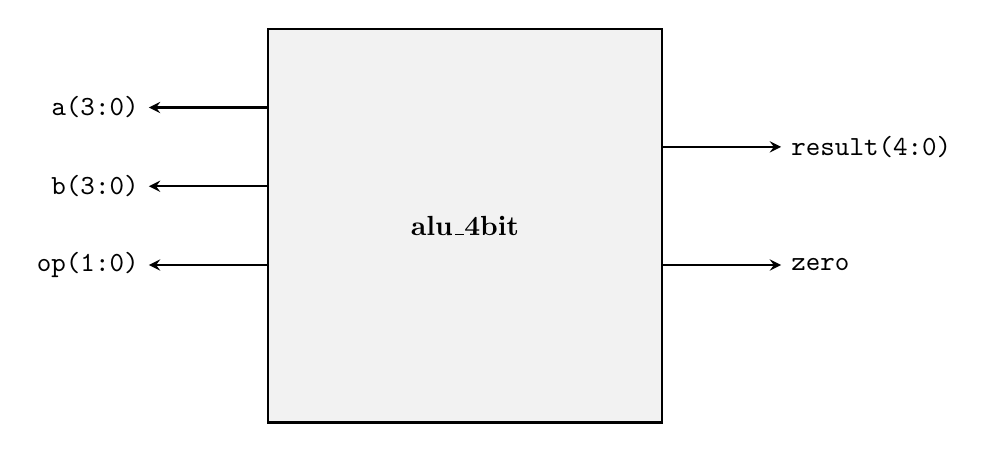
\begin{tikzpicture}[auto, node distance=1.5cm, >=stealth]
  \node[draw, minimum width=5cm, minimum height=5cm, thick, fill=gray!10] (alu) {\textbf{alu\_4bit}};

  \draw[->, thick] (alu.west|-0,1.5) -- ++(-1.5,0) node[left] {\texttt{a(3:0)}};
  \draw[->, thick] (alu.west|-0,0.5) -- ++(-1.5,0) node[left] {\texttt{b(3:0)}};
  \draw[->, thick] (alu.west|-0,-0.5) -- ++(-1.5,0) node[left] {\texttt{op(1:0)}};

  \draw[->, thick] (alu.east|-0,1.0) -- ++(1.5,0) node[right] {\texttt{result(4:0)}};
  \draw[->, thick] (alu.east|-0,-0.5) -- ++(1.5,0) node[right] {\texttt{zero}};
\end{tikzpicture}
\caption{4位ALU顶层端口框图}
\end{figure}

\textbf{评分标准：}5个端口全部标注且方向正确（2分），位宽标注正确（2分）。

\subsubsection*{（2）ALU功能表（3分）}

\begin{table}[h]
\centering
\caption{4位ALU功能表}
\begin{tabular}{|c|c|c|c|}
\hline
\textbf{op(1:0)} & \textbf{运算} & \textbf{输出表达式} & \textbf{result各位来源} \\
\hline
00 & 加法 & result = a + b & result(4)为进位，result(3:0)为和 \\
01 & 减法 & result = a - b & result(4)为借位，result(3:0)为差 \\
10 & 按位与 & result = `0' \& (a AND b) & result(4)=0，result(3:0)=a AND b \\
11 & 按位或 & result = `0' \& (a OR b) & result(4)=0，result(3:0)=a OR b \\
\hline
\end{tabular}
\end{table}

\textbf{评分标准：}4种运算的描述及表达式正确（2分），result位来源说明正确（1分）。

\subsubsection*{（3）VHDL代码（10分）}

\begin{lstlisting}[language=VHDL, numbers=left, caption={4位ALU（数据流描述风格）}]
-- ============================================================
-- 模块名：alu_4bit
-- 功能  ：4位算术逻辑单元
-- 操作  ：op=00(加), 01(减), 10(与), 11(或)
-- 说明  ：算术运算result(4)为进位/借位；逻辑运算result(4)='0'
--        result(4:0)共5位, zero标志检测result(3:0)=0
-- ============================================================
LIBRARY IEEE;
USE IEEE.STD_LOGIC_1164.ALL;
USE IEEE.NUMERIC_STD.ALL;

ENTITY alu_4bit IS
  PORT(
    a      : IN  STD_LOGIC_VECTOR(3 DOWNTO 0);
    b      : IN  STD_LOGIC_VECTOR(3 DOWNTO 0);
    op     : IN  STD_LOGIC_VECTOR(1 DOWNTO 0);
    result : OUT STD_LOGIC_VECTOR(4 DOWNTO 0);  -- 5位：含进位/借位
    zero   : OUT STD_LOGIC
  );
END ENTITY alu_4bit;

ARCHITECTURE dataflow OF alu_4bit IS
  SIGNAL res_int : STD_LOGIC_VECTOR(4 DOWNTO 0);
BEGIN
  -- 使用WITH...SELECT实现运算选择
  WITH op SELECT
    res_int <=
      -- 加法：0 & a + 0 & b → 5位结果（含进位）
      STD_LOGIC_VECTOR( ('0' & UNSIGNED(a)) + ('0' & UNSIGNED(b)) ) WHEN "00",
      -- 减法：0 & a - 0 & b → 5位结果（含借位）
      STD_LOGIC_VECTOR( ('0' & UNSIGNED(a)) - ('0' & UNSIGNED(b)) ) WHEN "01",
      -- 按位与：高位补0
      '0' & (a AND b)                                             WHEN "10",
      -- 按位或：高位补0
      '0' & (a OR b)                                              WHEN "11",
      (OTHERS => '0')                                             WHEN OTHERS;

  result <= res_int;

  -- 零标志位：当result(3 DOWNTO 0) = "0000"时输出'1'
  zero <= '1' WHEN res_int(3 DOWNTO 0) = "0000" ELSE '0';

END ARCHITECTURE dataflow;
\end{lstlisting}

\textbf{评分标准（10分）：}
\begin{itemize}
  \item 实体定义完整，端口位宽和方向正确\hfill（2分）
  \item 使用WITH...SELECT或WHEN...ELSE实现数据流风格\hfill（1.5分）
  \item 加法实现正确（含高位扩展和类型转换）\hfill（1.5分）
  \item 减法实现正确\hfill（1.5分）
  \item 按位与/或实现正确，高位补0\hfill（1.5分）
  \item 零标志位独立并发赋值语句生成\hfill（1分）
  \item 代码规范与注释\hfill（1分）
\end{itemize}

\subsubsection*{（4）注释说明（3分）}

\textbf{（1）算术与逻辑运算的不同处理方式：}
\begin{itemize}
  \item 算术运算（加减法）需要将\texttt{STD\_LOGIC\_VECTOR}转换为\texttt{UNSIGNED}类型，因为\texttt{+/-}运算符对\texttt{STD\_LOGIC\_VECTOR}未定义。同时需要在操作数前补`0'扩展为5位，以便容纳进位/借位。
  \item 逻辑运算（AND/OR）可直接对\texttt{STD\_LOGIC\_VECTOR}按位操作，结果高位补`0'组成5位输出。
\end{itemize}

\textbf{（2）result位宽设为5位的原因：}4位加法/减法可能产生进位或借位（超出4位表示范围），需要第5位（result(4)）来存储该进位/借位标志，保证结果不丢失信息。

\textbf{评分标准：}（1）说明正确（1.5分），（2）说明正确（1.5分）。

\newpage

% ============================================================
\subsection*{设计题2：参数化模N计数器设计（20分）}

\subsubsection*{（1）GENERIC声明与意义（3分）}

\begin{lstlisting}[language=VHDL]
ENTITY mod_n_counter IS
  GENERIC (N : INTEGER := 10);     -- 模值参数，默认10
  PORT( ... );
END ENTITY;
\end{lstlisting}

\textbf{GENERIC的意义：}
\begin{itemize}
  \item \textbf{参数化设计：}通过修改GENERIC值可使同一VHDL设计适配不同计数模值（如N=6、N=10、N=60），无需重写代码。
  \item \textbf{代码复用：}顶层模块在例化时通过\texttt{GENERIC MAP}传递实际参数值。
  \item \textbf{可维护性：}一处修改即可改变整体设计行为，便于调试和迭代。
\end{itemize}
\textbf{评分标准：}GENERIC声明语法正确（1.5分），意义说明充分（1.5分）。

\subsubsection*{（2）状态转移图（N=6）（5分）}

\begin{figure}[h]
\centering
\begin{tikzpicture}[->, >=stealth, auto, node distance=2cm, semithick,
  every state/.style={draw, circle, minimum width=1.2cm, fill=gray!10}]

  \node[state, initial below, initial text={rst}] (S0) {0\\tc=0};
  \node[state] (S1) [right of=S0] {1\\tc=0};
  \node[state] (S2) [right of=S1] {2\\tc=0};
  \node[state] (S3) [below of=S1] {3\\tc=0};
  \node[state] (S4) [left of=S3] {4\\tc=0};
  \node[state, fill=green!15] (S5) [right of=S3] {5\\tc=1};

  \path (S0) edge[bend left] node[above]{en=1} (S1)
             edge[loop above] node{en=0} (S0)
        (S1) edge[bend left] node[above]{en=1} (S2)
             edge[loop above] node{en=0} (S1)
        (S2) edge[bend left] node[below]{en=1} (S3)
             edge[loop above] node{en=0} (S2)
        (S3) edge[bend left] node[below]{en=1} (S4)
             edge[loop above] node{en=0} (S3)
        (S4) edge[bend left] node[below]{en=1} (S5)
             edge[loop above] node{en=0} (S4)
        (S5) edge[bend left=60] node[left]{en=1} (S0)
             edge[loop above] node{en=0} (S5);
\end{tikzpicture}
\caption{模6计数器状态转移图（0--5，tc仅在状态5时为1）}
\end{figure}

\textbf{评分标准：}6个状态齐全（1.5分），转移条件正确（en=1前进/en=0保持）（2分），tc输出标注正确（仅S5时tc=1）（1.5分）。

\subsubsection*{（3）VHDL代码（9分）}

\begin{lstlisting}[language=VHDL, numbers=left, caption={参数化模N计数器（行为描述）}]
-- ============================================================
-- 模块名：mod_n_counter
-- 功能  ：参数化模N同步计数器（0 ~ N-1）
-- 说明  ：GENERIC N控制模值；同步复位>使能优先级
--        tc在计数值=N-1且en='1'时输出'1'
-- ============================================================
LIBRARY IEEE;
USE IEEE.STD_LOGIC_1164.ALL;
USE IEEE.NUMERIC_STD.ALL;

ENTITY mod_n_counter IS
  GENERIC (N : INTEGER := 10);              -- 模值参数
  PORT(
    clk : IN  STD_LOGIC;
    rst : IN  STD_LOGIC;                    -- 同步复位，高有效
    en  : IN  STD_LOGIC;                    -- 计数使能，高有效
    q   : OUT STD_LOGIC_VECTOR(3 DOWNTO 0); -- 计数值输出
    tc  : OUT STD_LOGIC                     -- 终端计数
  );
END ENTITY mod_n_counter;

ARCHITECTURE behav OF mod_n_counter IS
  SIGNAL count : INTEGER RANGE 0 TO N-1 := 0;  -- 内部计数器
BEGIN
  PROCESS(clk)
  BEGIN
    IF rising_edge(clk) THEN
      IF rst = '1' THEN                     -- 同步复位（最高优先级）
        count <= 0;
      ELSIF en = '1' THEN                   -- 使能控制
        IF count = N-1 THEN
          count <= 0;                       -- 计满回零
        ELSE
          count <= count + 1;
        END IF;
      END IF;                               -- en=0时保持
    END IF;
  END PROCESS;

  -- 输出转换
  q  <= STD_LOGIC_VECTOR(TO_UNSIGNED(count, 4));

  -- 终端计数：count=N-1且en='1'时tc=1
  tc <= '1' WHEN (count = N-1) AND (en = '1') ELSE '0';

END ARCHITECTURE behav;
\end{lstlisting}

\textbf{评分标准（9分）：}
\begin{itemize}
  \item GENERIC定义正确（INTEGER类型，默认值10）\hfill（1分）
  \item 内部INTEGER信号定义正确（范围0 TO N-1）\hfill（1分）
  \item 同步复位实现正确（仅IF rising\_edge内判断）\hfill（1.5分）
  \item 使能控制逻辑正确（en=1时计数，en=0时保持）\hfill（1.5分）
  \item 模N回零逻辑正确（count=N-1→0）\hfill（1.5分）
  \item tc输出逻辑正确（count=N-1且en=1时有效）\hfill（1.5分）
  \item 代码规范与注释\hfill（1分）
\end{itemize}

\subsubsection*{（4）问题回答（3分）}

\textbf{（a）N=60时端口适配问题（1.5分）：}4位输出的\texttt{q(3 DOWNTO 0)}最大可表示$2^4-1=15$，无法完整表示计数值$0\sim59$。需将\texttt{q}的位宽从4位扩展为6位（\texttt{q(5 DOWNTO 0)}，$2^6=64\ge60$），并将输出转换语句中的位宽参数改为6：\texttt{TO\_UNSIGNED(count, 6)}。

\textbf{（b）同步复位与异步复位的优缺点对比（1.5分）：}

\begin{table}[h]
\centering
\begin{tabular}{|p{0.22\textwidth}|p{0.35\textwidth}|p{0.35\textwidth}|}
\hline
\textbf{对比维度} & \textbf{同步复位} & \textbf{异步复位} \\
\hline
复位响应 & 仅在时钟沿生效，可能延迟1周期 & 立即生效，不等待时钟 \\
\hline
时序稳定性 & 好，复位与时钟同步，无亚稳态风险 & 需处理复位释放时的恢复时间问题 \\
\hline
资源占用 & 略多（复位信号需经过数据路径） & 可使用触发器专用复位端，资源少 \\
\hline
\end{tabular}
\end{table}

\textbf{改用异步复位的代码修改：}
\begin{enumerate}
  \item PROCESS敏感信号表添加\texttt{rst}：\texttt{PROCESS(clk, rst)}
  \item 将复位判断移至\texttt{IF rising\_edge(clk)}之前：

\begin{lstlisting}[language=VHDL]
PROCESS(clk, rst)
BEGIN
  IF rst = '1' THEN
    count <= 0;            -- 异步复位
  ELSIF rising_edge(clk) THEN
    IF en = '1' THEN
      IF count = N-1 THEN
        count <= 0;
      ELSE
        count <= count + 1;
      END IF;
    END IF;
  END IF;
END PROCESS;
\end{lstlisting}
\end{enumerate}

\textbf{评分标准：}（a）正确指出4位不够并给出正确修改方案（1.5分）；（b）优缺点对比合理（0.75分），异步复位代码修改正确（0.75分）。

\newpage

% ============================================================
\subsection*{设计题3：电子密码锁控制器（20分）}

\subsubsection*{（1）状态定义与状态转移图（4分）}

\textbf{状态定义（Moore型）：}
\begin{itemize}
  \item \textbf{S0（IDLE/初始）：}未匹配任何位，等待首位输入。unlock=0。
  \item \textbf{S1（已匹配``1''）：}已正确输入密码第1位`1'。unlock=0。
  \item \textbf{S2（已匹配``11''）：}已正确输入密码前2位``11''。unlock=0。
  \item \textbf{S3（已匹配``110''）：}已正确输入密码前3位``110''。unlock=0。
  \item \textbf{S4（已匹配``1101''——开锁）：}4位密码全部匹配。unlock=1。
\end{itemize}

\textbf{状态机类型：Moore型}——unlock仅由当前状态决定（仅S4时unlock=1），与输入din无关。

\begin{figure}[h]
\centering
\begin{tikzpicture}[->, >=stealth, auto, node distance=2.8cm, semithick,
  every state/.style={draw, rectangle, rounded corners, minimum width=2.2cm, minimum height=0.9cm, fill=gray!10}]

  \node[state, initial below, initial text={复位}, fill=blue!10] (S0) {S0(IDLE)\\unlock=0};
  \node[state] (S1) [right of=S0] {S1\\unlock=0};
  \node[state] (S2) [right of=S1] {S2\\unlock=0};
  \node[state] (S3) [right of=S2] {S3\\unlock=0};
  \node[state, fill=green!15] (S4) [below of=S2, yshift=-1.5cm] {S4\\unlock=1};

  \path (S0) edge[loop above] node{din=0} (S0)
             edge[bend left] node[above]{din=1} (S1)
        (S1) edge[loop above] node{din=0} (S0)  % Actually wrong: din=0 in S1 goes to S0
             % Let me fix: din=1 in S1 stays S1 or goes to S2
        % The actual transitions:
        % S0: din=0→S0, din=1→S1
        % S1: din=0→S0, din=1→S2
        % S2: din=0→S3, din=1→S0
        % S3: din=0→S0, din=1→S4
        % S4: unconditionally→S0
\end{tikzpicture}
\caption{电子密码锁Moore型状态转移图}
\end{figure}

\textbf{注：}为完整展示所有转移——图中各状态转移条件可描述为：
\begin{itemize}
  \item S0 $\xrightarrow{\text{din=1}}$ S1（匹配`1'）；S0 $\xrightarrow{\text{din=0}}$ S0（等待）
  \item S1 $\xrightarrow{\text{din=1}}$ S2（匹配``11''）；S1 $\xrightarrow{\text{din=0}}$ S0（不匹配，回初始）
  \item S2 $\xrightarrow{\text{din=0}}$ S3（匹配``110''）；S2 $\xrightarrow{\text{din=1}}$ S0（不匹配）
  \item S3 $\xrightarrow{\text{din=1}}$ S4（匹配``1101''）；S3 $\xrightarrow{\text{din=0}}$ S0（不匹配）
  \item S4 $\xrightarrow{\text{无条件}}$ S0（开锁后返回初始，非重叠检测）
\end{itemize}

\textbf{评分标准（4分）：}
\begin{itemize}
  \item 5个状态定义清晰、含义正确\hfill（1.5分）
  \item 所有转移条件完整正确（10条弧）\hfill（1.5分）
  \item 各状态unlock输出标注正确（仅S4=1）\hfill（0.5分）
  \item 注明Moore型及理由\hfill（0.5分）
\end{itemize}

\subsubsection*{（2）状态转移表（4分）}

\begin{table}[h]
\centering
\caption{密码锁Moore型状态转移表（密码：1101，非重叠检测）}
\begin{tabular}{|c|c|c|c|}
\hline
\textbf{当前状态} & \textbf{din} & \textbf{次态} & \textbf{unlock} \\
\hline
S0(IDLE) & 0 & S0 & 0 \\
S0(IDLE) & 1 & S1 & 0 \\
\hline
S1(已匹配``1'') & 0 & S0 & 0 \\
S1(已匹配``1'') & 1 & S2 & 0 \\
\hline
S2(已匹配``11'') & 0 & S3 & 0 \\
S2(已匹配``11'') & 1 & S0 & 0 \\
\hline
S3(已匹配``110'') & 0 & S0 & 0 \\
S3(已匹配``110'') & 1 & S4 & 0 \\
\hline
S4(已匹配``1101'') & $\times$ & S0 & 1 \\
\hline
\end{tabular}
\end{table}

\textbf{评分标准：}表格完整覆盖所有状态和输入（2分），次态全部正确（1.5分），unlock列正确（0.5分）。

\subsubsection*{（3）VHDL代码（9分）}

\begin{lstlisting}[language=VHDL, numbers=left, caption={电子密码锁控制器（双进程Moore型，密码1101）}]
-- ============================================================
-- 模块名：password_lock
-- 功能  ：电子密码锁控制器（Moore型，密码固定为"1101"）
-- 说明  ：非重叠检测——开锁后立即回到S0重新检测
--        din每次输入1位, 连续4位匹配"1101"则unlock=1
-- ============================================================
LIBRARY IEEE;
USE IEEE.STD_LOGIC_1164.ALL;

ENTITY password_lock IS
  PORT(
    clk    : IN  STD_LOGIC;
    rst    : IN  STD_LOGIC;           -- 异步复位，高有效
    din    : IN  STD_LOGIC;           -- 串行密码输入(1位/周期)
    unlock : OUT STD_LOGIC            -- 开锁信号
  );
END ENTITY password_lock;

ARCHITECTURE fsm OF password_lock IS
  -- 自定义枚举类型：S0=IDLE, S1~S4=已匹配1~4位
  TYPE lock_state IS (S0, S1, S2, S3, S4);
  SIGNAL current_state, next_state : lock_state;
BEGIN

  -- ====== 时序进程：状态寄存器 + 异步复位 ======
  PROCESS(clk, rst)
  BEGIN
    IF rst = '1' THEN
      current_state <= S0;            -- 异步复位回到IDLE
    ELSIF rising_edge(clk) THEN
      current_state <= next_state;
    END IF;
  END PROCESS;

  -- ====== 组合进程：次态逻辑 ======
  PROCESS(current_state, din)
  BEGIN
    -- 默认值
    next_state <= S0;

    CASE current_state IS
      WHEN S0 =>                      -- IDLE：等待首位输入
        IF din = '1' THEN
          next_state <= S1;           -- 匹配密码第1位'1'
        ELSE
          next_state <= S0;           -- din='0'→继续等待
        END IF;

      WHEN S1 =>                      -- 已匹配"1"
        IF din = '1' THEN
          next_state <= S2;           -- 匹配密码第2位'1'→"11"
        ELSE
          next_state <= S0;           -- din='0'→不匹配，回IDLE
        END IF;

      WHEN S2 =>                      -- 已匹配"11"
        IF din = '0' THEN
          next_state <= S3;           -- 匹配密码第3位'0'→"110"
        ELSE
          next_state <= S0;           -- din='1'→不匹配
        END IF;

      WHEN S3 =>                      -- 已匹配"110"
        IF din = '1' THEN
          next_state <= S4;           -- 匹配密码第4位'1'→"1101"
        ELSE
          next_state <= S0;           -- din='0'→不匹配
        END IF;

      WHEN S4 =>                      -- 已匹配"1101"——开锁
        next_state <= S0;             -- 非重叠：开锁后回IDLE重新检测

      WHEN OTHERS =>
        next_state <= S0;
    END CASE;
  END PROCESS;

  -- ====== Moore型输出逻辑：unlock仅取决于当前状态 ======
  unlock <= '1' WHEN current_state = S4 ELSE '0';

END ARCHITECTURE fsm;
\end{lstlisting}

\textbf{评分标准（9分）：}
\begin{itemize}
  \item 枚举类型定义正确（TYPE lock\_state IS...）\hfill（1分）
  \item 双进程风格清晰（时序进程+组合进程分离）\hfill（1分）
  \item 异步复位正确（rst在敏感表，IF rst先于时钟判断）\hfill（1分）
  \item S0--S4次态逻辑全部正确（含不匹配回S0）\hfill（4分）\\（每个状态的匹配/不匹配逻辑各0.8分）
  \item Moore型输出逻辑正确（仅current\_state=S4时unlock=1）\hfill（1分）
  \item 代码注释清晰、说明各状态含义和关键转换条件\hfill（1分）
\end{itemize}

\subsubsection*{（4）问题回答（3分）}

\textbf{（a）Moore型与Mealy型在密码锁应用中的区别（1.5分）：}

\begin{itemize}
  \item \textbf{Moore型：}unlock输出仅取决于当前状态。只有进入S4后unlock才为1，输出与时钟同步变化。在本设计中，密码第4位din=1的时钟上升沿后，状态变为S4，unlock在此时钟周期内为1。
  \item \textbf{Mealy型：}unlock输出取决于当前状态\textbf{和}当前输入din。若改用Mealy型实现，当状态为S3且din=1时，unlock可\textbf{立即}为1（组合逻辑输出），比Moore型提前一个时钟周期响应。但Mealy型的输出可能产生毛刺（glitch），在密码锁等安全关键应用中需谨慎。
\end{itemize}

\textbf{（b）支持密码可修改的扩展方案（1.5分）：}

\textbf{需增加的输入端口：}
\begin{itemize}
  \item \texttt{prog\_mode}（1位）：编程模式使能
  \item \texttt{new\_din(3 DOWNTO 0)}（4位）：新密码并行输入（或串行方案：增加\texttt{prog\_din}（1位）逐位输入）
  \item \texttt{prog\_clk}或使用现有clk配合\texttt{prog\_mode}实现时序控制
\end{itemize}

\textbf{状态机主要改动：}
\begin{enumerate}
  \item 将固定密码``1101''替换为内部寄存器\texttt{password\_reg(3 DOWNTO 0)}，在编程模式下可被写入。
  \item 增加编程状态（如PROG\_S0--PROG\_S3），在\texttt{prog\_mode=1}时进入编程流程，逐位存储新密码。
  \item 比较逻辑改为：将当前输入din与\texttt{password\_reg}的对应位逐一比对（而非硬编码``1101''）。
  \item 增加密码存储的非易失性支持（如EEPROM写入逻辑，或至少保持到下次编程）。
\end{enumerate}

\textbf{评分标准：}（a）Moore与Mealy区别描述正确（1.5分）；（b）端口增加方案合理（0.75分），状态机改动方向正确（0.75分）。

\vspace{0.5cm}
{\centering
\rule{0.8\textwidth}{0.5pt}
\vspace{0.3cm}

\textbf{—— 第12套参考答案结束 ——}

\vspace{0.5cm}}

\endinput
